\documentclass[11pt]{beamer}
% \usetheme{Boadilla}
  \usetheme{default}


% acronyms for text or math mode
\newcommand {\ccast} {\mbox{\small CCAST}}
\newcommand {\cris} {\mbox{\small CrIS}}

\newcommand {\airs} {\mbox{\small AIRS}}
\newcommand {\iasi} {\mbox{\small IASI}}
\newcommand {\idps} {\mbox{\small IDPS}}
\newcommand {\nasa} {\mbox{\small NASA}}
\newcommand {\noaa} {\mbox{\small NOAA}}
\newcommand {\nstar} {\mbox{\small STAR}}
\newcommand {\umbc} {\mbox{\small UMBC}}
\newcommand {\uw}   {\mbox{\small UW}}

\newcommand {\fft}  {\mbox{\small FFT}}
\newcommand {\ifft} {\mbox{\small IFFT}}
\newcommand {\fir}  {\mbox{\small FIR}}
\newcommand {\fov}  {\mbox{\small FOV}}
\newcommand {\for}  {\mbox{\small FOR}}
\newcommand {\ict}  {\mbox{\small ICT}}
\newcommand {\ils}  {\mbox{\small ILS}}
\newcommand {\igm}  {\mbox{\small IGM}}
\newcommand {\opd}  {\mbox{\small OPD}}
\newcommand {\rms}  {\mbox{\small RMS}}
\newcommand {\zpd}  {\mbox{\small ZPD}}
\newcommand {\ppm}  {\mbox{\small PPM}}
\newcommand {\srf}  {\mbox{\small SRF}}

\newcommand {\ES} {\mbox{\small ES}}
\newcommand {\SP} {\mbox{\small SP}}
\newcommand {\IT} {\mbox{\small IT}}
\newcommand {\SA} {\mbox{\small SA}}

\newcommand {\ET} {\mbox{\small ET}}
\newcommand {\FT} {\mbox{\small FT}}

% abbreviations, mainly for math mode
\newcommand {\real} {\mbox{real}}
\newcommand {\imag} {\mbox{imag}}
\newcommand {\atan} {\mbox{atan}}
\newcommand {\obs}  {\mbox{obs}}
\newcommand {\calc} {\mbox{calc}}
\newcommand {\sinc} {\mbox{sinc}}
\newcommand {\psinc} {\mbox{psinc}}
\newcommand {\std} {\mbox{std}}

% symbols, for math mode only
\newcommand {\wnum} {\mbox{cm$^{-1}$}}
\newcommand {\lmax} {L_{\mbox{\tiny max}}}
\newcommand {\vmax} {V_{\mbox{\tiny max}}}

\newcommand {\tauobs} {\tau_{\mbox{\tiny obs}}}
\newcommand {\taucal} {\tau_{\mbox{\tiny calc}}}
\newcommand {\Vdc}  {V_{\mbox{\tiny DC}}}

\newcommand {\rIT} {r_{\mbox{\tiny\textsc{ict}}}}
\newcommand {\rES} {r_{\mbox{\tiny\textsc{es}}}}
\newcommand {\robs} {r_{\mbox{\tiny obs}}}

\newcommand {\rITobs} {r_{\mbox{\tiny\textsc{ict}}}^{\mbox{\tiny obs}}}
\newcommand {\rITcal} {r_{\mbox{\tiny\textsc{ict}}}^{\mbox{\tiny cal}}}

\newcommand {\ITmean} {\langle\mbox{\small IT}\rangle}
\newcommand {\SPmean} {\langle\mbox{\small SP}\rangle}


\title{ccast calibration equations}
\author{H.~E.~Motteler and L.~L.~Strow}
\institute{
  UMBC Atmospheric Spectroscopy Lab \\
  Joint Center for Earth Systems Technology \\
}
\date{\today}
\begin{document}

%----------- slide --------------------------------------------------%
\begin{frame}[plain]
\titlepage
\end{frame}
%----------- slide --------------------------------------------------%
\begin{frame}
\frametitle{introduction}

An overview of the {\umbc} {\ccast} calibration equations,
parameters, filters, and {\ils}.  Topics include

\vspace{3mm}
\begin{itemize}

  \item {\ccast} and {\noaa} calibration equations
  \item calibration equation parameters
  \item \ccast\ \cris\ resolution modes
  \item raised cosine and \atbd\ processing filters
  \item processing, {\fir} filter, and responsivity plots
  \item {\ccast} {\ils} with sample plots
  \item extended resolution apodization

\end{itemize}

\end{frame}
%----------- slide --------------------------------------------------%
\begin{frame}
\frametitle{ccast calibration equations}

% \begin{equation}
%   \rES = F \cdot \rIT \cdot f \cdot \SA^{-1}\cdot f \cdot 
%          \frac{\ES - \SPmean}{\ITmean - \SPmean}
% \end{equation}

\begin{center}
{\ccast} reference equation
\end{center}
\vspace{-2mm}
\begin{equation}
  \rESuser = F \cdot \rITsensor \cdot \fcos \cdot \SA^{-1}\cdot \fcos 
         \cdot \frac{\Delta\ES}{\Delta\IT}
\end{equation}

\begin{equation}
  \rESuser = F \cdot \fcos \cdot \SA^{-1}\cdot \fcos \cdot \rITfov 
         \cdot \frac{\Delta\ES}{\Delta\IT}
\end{equation}

\vspace{3mm}
\begin{center}
{\noaa} algorithm 4
\end{center}
\vspace{-2mm}
\begin{equation}
  \rESuser = \rITuser \cdot
         \frac{F \cdot \fatbd \cdot \SA^{-1}\cdot \fatbd \cdot 
                  (\frac{\Delta\ES}{\Delta\IT}) \cdot {|\Delta\IT|}}
              {F \cdot \fatbd \cdot \SA^{-1}\cdot \fatbd \cdot {|\Delta\IT|}}
\end{equation}

\vspace{3mm}
\[ \Delta\ES = \ES - \SPmean, \hspace{4mm}
   \Delta\IT = \ITmean - \SPmean \]

\end{frame}
%----------- slide --------------------------------------------------%
\begin{frame}
\frametitle{calibration equation parameters}

\vspace{-8mm}
\begin{align*}
  \ES &= \mbox{\small NLC}(\fir^{-1}(\ES_0)) \\
  \ITmean &= \mbox{\small NLC}(\fir^{-1}(\langle\IT_0\rangle)) \\
  \SPmean &= \mbox{\small NLC}(\fir^{-1}(\langle\SP_0\rangle)) \\
\end{align*}
\vspace{-8mm}

{\small NLC} is the ATBD non-linearity correction and $\ES_0$,
$\IT_0$, and $\SP_0$ are uncorrected earth-scene, ICT, and space
spectra.  $\langle\IT_0\rangle$ and $\langle\SP_0\rangle$ are moving
averages, by default over 9 scans.  $\fir^{-1}$ is pointwise division
by the spectral form of the numeric filter

\begin{itemize}
  \item $\rITuser$ is expected ICT radiance at the user grid
  \item $\rITsensor$ is expected ICT radiance at the sensor grid
  \item $\rITfov = \SA \cdot \rITsensor$, expected uncorrected ICT
    radiance 
\end{itemize}

\end{frame}
%----------- slide --------------------------------------------------%
\begin{frame}
\frametitle{calibration equation parameters}

expected ICT radiance is calculated as per the ATBD, using
engineering packet parameters and a scan baffle temperature orbit
profile correction

\begin{itemize}
  \item $\rESuser$ is calibrated earth-scene radiance at the user grid
  \item $F$ is double Fourier interpolation from sensor to user grid
  \item $\fcos$ is a raised-cosine bandpass filter with wings at or just
    inside instrument responsivity
  \item $\fatbd$ is the {\noaa} version of the {\cris} ATBD expontial
    bandpass filter
  \item the columns of $\SA$ are the periodic sinc ILS wrapping at
    the sensor grid, without extension or trimming

\end{itemize}

\end{frame}
%----------- slide --------------------------------------------------%
\begin{frame}
\frametitle{\ccast\ resolution modes}

\begin{itemize}

  \item \umbc\ \ccast\ sensor-grid resolution modes include

\begin{tabular}{crrrl}
   mode  &  LW  &   MW  &  SW  &  comment  \\
   \hline
  lowres &  866 &   530 &  202 &  low res  \\
  hires1 &  866 &  1039 &  799 &  old high res  \\
  hires2 &  866 &  1052 &  799 &  2014 high res  \\
  hi3to2 &  866 &  1052 &  800 &  truncation test  \\
  hires3 &  874 &  1052 &  808 &  new extended res  \\
\end{tabular}

  \item {\ccast} user grid resolution modes include the original
    0.8/0.4/0.2 {\wn} {\opd} low res mode and the 0.8 {\wn}
    {\opd} high res mode

  \item double Fourier interpolation from the sensor to user grid
    allows for any combination of sensor and user resolutions

  \item interferogram centers are at decimated points $n/2 + 1$
    for even point sets.  The center is at $n/2 + 1$ for the 799
    point set as well, but in that case is not an integer

\end{itemize}

\end{frame}
%----------- slide --------------------------------------------------%
\begin{frame}
\frametitle{raised cosine processing filter}

{\ccast} processing filter weight as a function of frequency is

\[
  \fcos(v) = 
    \begin{cases}
      \hspace{4pt} 0                               &  v < v_L \\
      (1 + \cos(-\pi (p_L - v) / (p_L - v_L))) / 2  &  v_L \leq v < p_L \\
      \hspace{4pt} 1                               &  p_L \leq v < p_H \\
      (1 + \cos( \pi (p_H - v) / (p_L - v_H))) / 2  &  p_H \leq v < v_H \\
      \hspace{4pt} 0                               &  v_H \leq v
    \end{cases}
\]

{\ccast} high res filter parameters are

\vspace{3mm}
\begin{tabular}{crrrrrrr}
band &  $p_L$ &  $p_H$ &  $r_L$ & $r_H$ \\
LW   &   650  &  1100  &   15  &  20  \\
MW   &  1200  &  1760  &   30  &  30  \\
SW   &  2145  &  2560  &   30  &  30
\end{tabular}

\vspace{4mm}

with $v_L = p_L - r_L$ and $v_H = p_H + r_H$

\end{frame}
%----------- slide --------------------------------------------------%
\begin{frame}
\frametitle{\atbd\ processing filter}

{\atbd} processing filter weights as a function of index are

\[
  \fatbd(k) = \frac{1}{e^{a_2 (k_0-a_1-k)} + 1} \cdot
               \frac{1}{e^{a_4 (k-k_1-a_3)} + 1}
\]

% a = [np; k0; k1; a1; a2; a3; a4];
% fprintf(1, '%5d%5d%5d%5d%6.2f%5d%6.2f\n', a)

\vspace{2mm}

NOAA high res ATBD filter parameters \\
\vspace{2mm}
\begin{tabular}{crrrrrrr}
band & size  & $k_0$ & $k_1$ & $a_1$ & $a_2$ & $a_3$ & $a_4$ \\
LW   &  866  &  78 &  790 &  30 &  0.5 &  30 &  0.5 \\
MW   & 1052  &  95 &  959 &  59 &  0.5 &  59 &  0.5 \\
SW   &  799  &  84 &  716 &  41 &  0.5 &  41 &  0.5
\end{tabular}

\vspace{4mm}
UMBC extended res ATBD filter parameters \\
\vspace{2mm}
\begin{tabular}{crrrrrrr}
band & size  & $k_0$ & $k_1$ & $a_1$ & $a_2$ & $a_3$ & $a_4$ \\
LW   &  874  &  79 &  797 &  30 &  0.5 &  30 &  0.5 \\
MW   & 1052  &  95 &  959 &  59 &  0.5 &  59 &  0.5 \\
SW   &  808  &  85 &  724 &  41 &  0.5 &  41 &  0.5
\end{tabular}

\end{frame}
%----------- slide --------------------------------------------------%
\begin{frame}
\frametitle{ccast and noaa LW filters}
\begin{center}
  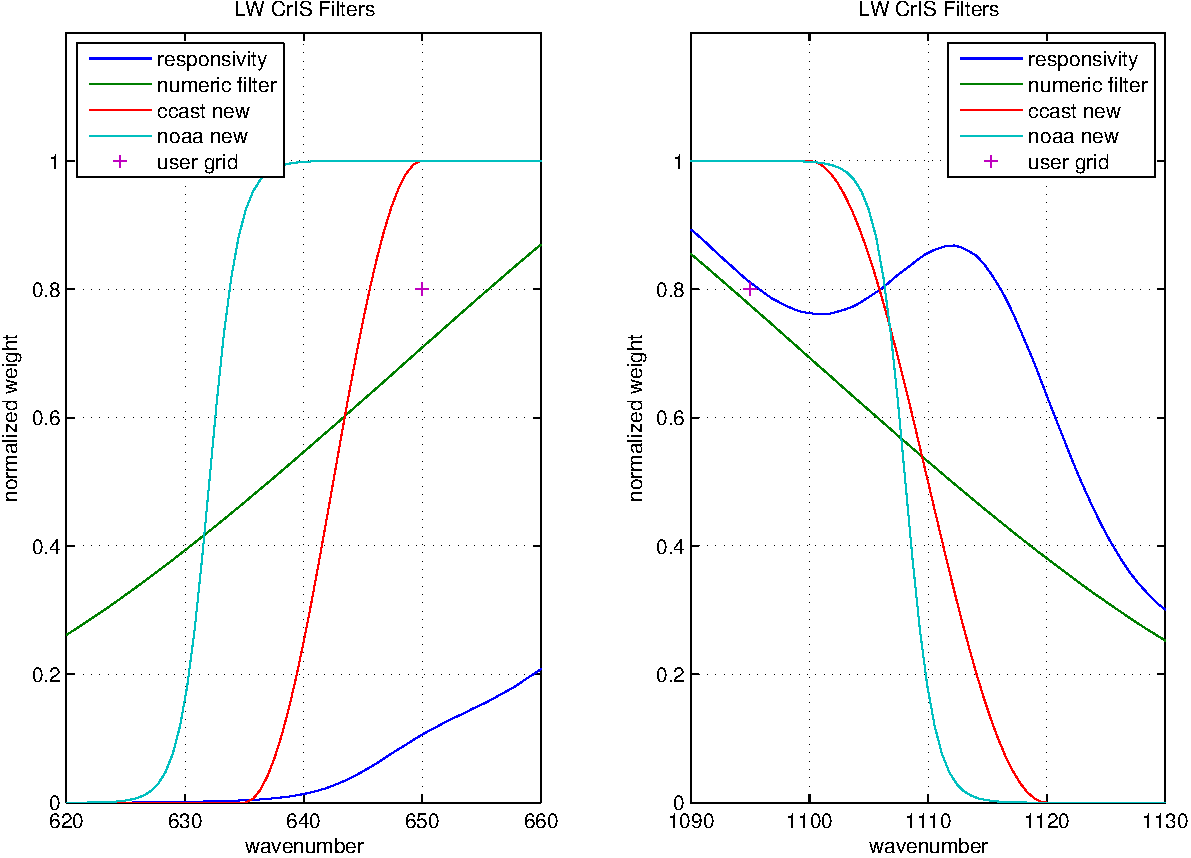
\includegraphics[scale=0.5]{figures/show_filts_LW.pdf}
\end{center}
\end{frame}
%----------- slide --------------------------------------------------%
\begin{frame}
\frametitle{ccast and noaa MW filters}
\begin{center}
  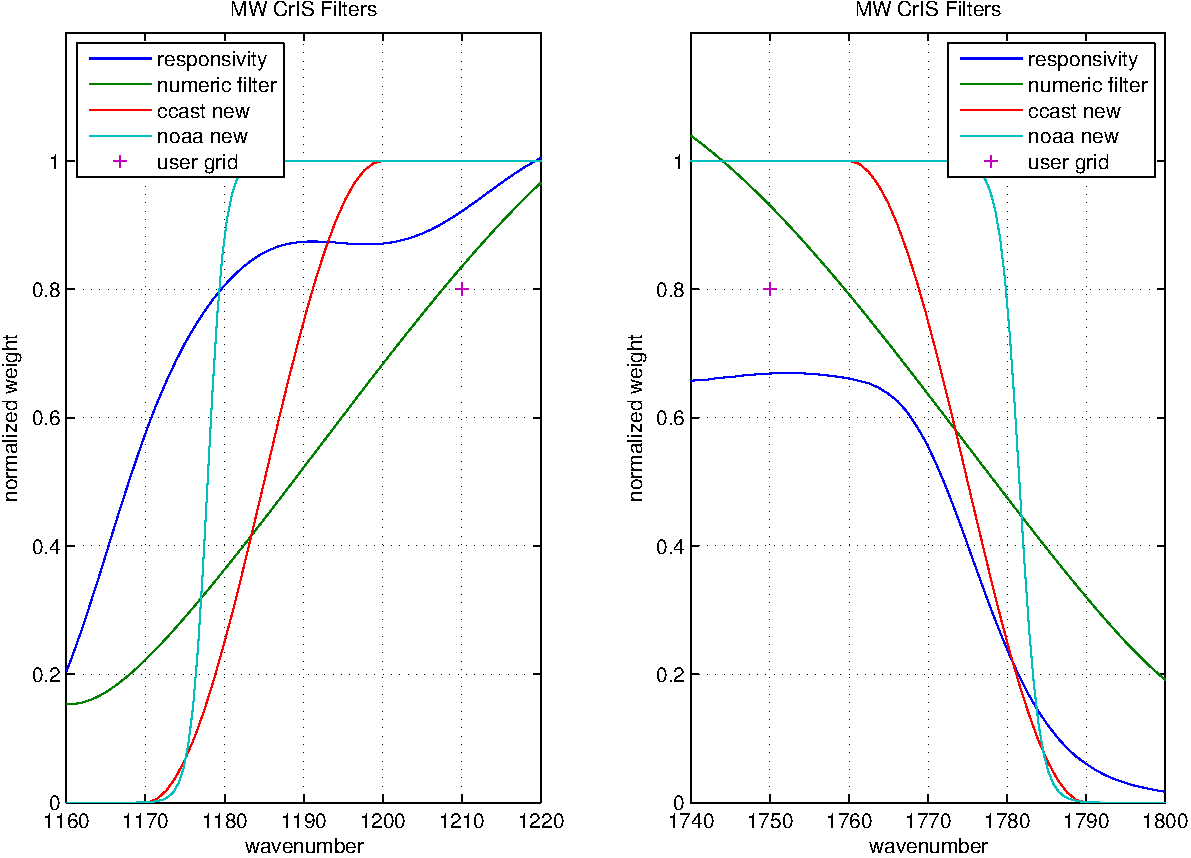
\includegraphics[scale=0.5]{figures/show_filts_MW.pdf}
\end{center}
\end{frame}
%----------- slide --------------------------------------------------%
\begin{frame}
\frametitle{ccast and noaa SW filters}
\begin{center}
  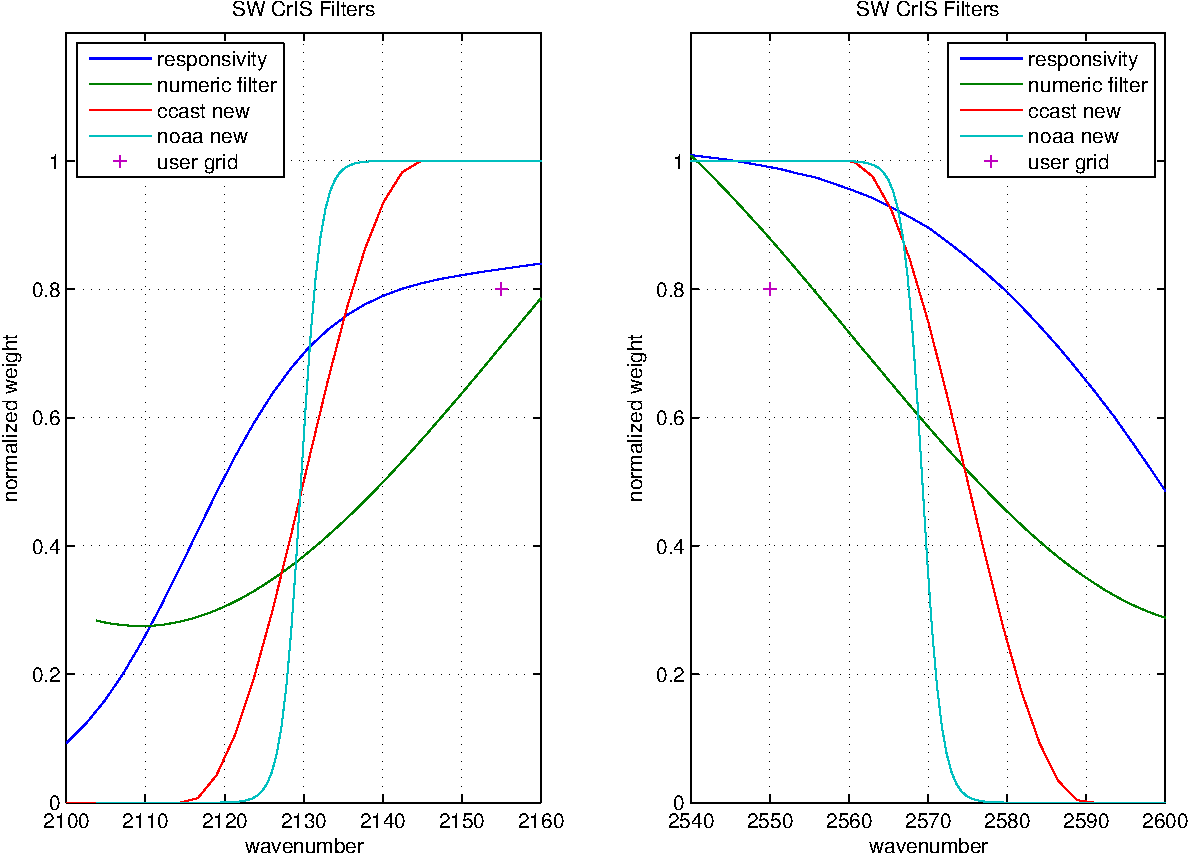
\includegraphics[scale=0.5]{figures/show_filts_SW.pdf}
\end{center}
\end{frame}
%----------- slide --------------------------------------------------%
\begin{frame}
\frametitle{\ccast\ \ils\ function}

the \ccast\ \ils\ for $\fov_i$ can be represented as

\[\int_{\mbox{\tiny FOV}_i} \!\!\!\! w_i(\theta)\, \psinc(2 \pi
                 d(v - v_0 \cos \theta ))\, d\theta \]

% f_{v_0}(v) = 
% \int_{\mbox{\tiny FOV}_i}
% \int_{a_i}^{b_i}

\begin{itemize}
  \item $d$ is max \opd
  \item $v$ is frequency
  \item $v_0$ is reference or channel frequency
  \item $\psinc(x) = sin(x)/(n \sin(x/n))$ for $x \ne 0$,  $1$ for
    $x = 0$, where $n$ is the number of points in the sensor grid
   \item $\psinc(2 \pi d(v - v_0 \cos \theta ))$ gives the ILS for a
    single ray at off-axis angle $\theta$
  \item integration is over the intersection of on-axis arcs with
    $\fov_i$, with $w_i(\theta)$ the length of an intersecting arc
    at off-axis angle $\theta$
\end{itemize}

\end{frame}
%----------- slide --------------------------------------------------%
\begin{frame}
\frametitle{\ccast\ \SA\ matrix}

the \ccast\ \SA\ matrix for $\fov_k$ is

\[\SA(i,j) = \int_{\mbox{\tiny FOV}_k} \!\!\!\! w_k(\theta)\, \psinc(2 \pi
                 \delta(v_i - v_j \cos \theta ))\, d\theta \]

\begin{itemize}
  \item $1 \le i,j \le n$, for $n$ the number of points in the
    sensor grid
  \item $v_i$ is frequency for channel $i$, and $\delta$ is max \opd
  \item $\psinc(x) = sin(x)/(n \sin(x/n))$ for $x \ne 0$,  $1$ for
    $x = 0$
   \item $\psinc(2 \pi \delta(v - v_0 \cos \theta ))$ gives the ILS
     for a single ray at off-axis angle $\theta$ and reference or
     channel frequency $v_0$
  \item integration is over the intersection of on-axis arcs with
    $\fov_k$, with $w_k(\theta)$ the length of an intersecting arc
    at off-axis angle $\theta$
\end{itemize}

\end{frame}
%----------- slide --------------------------------------------------%
\begin{frame}
\frametitle{sample \ccast\ \ils}
\begin{center}
  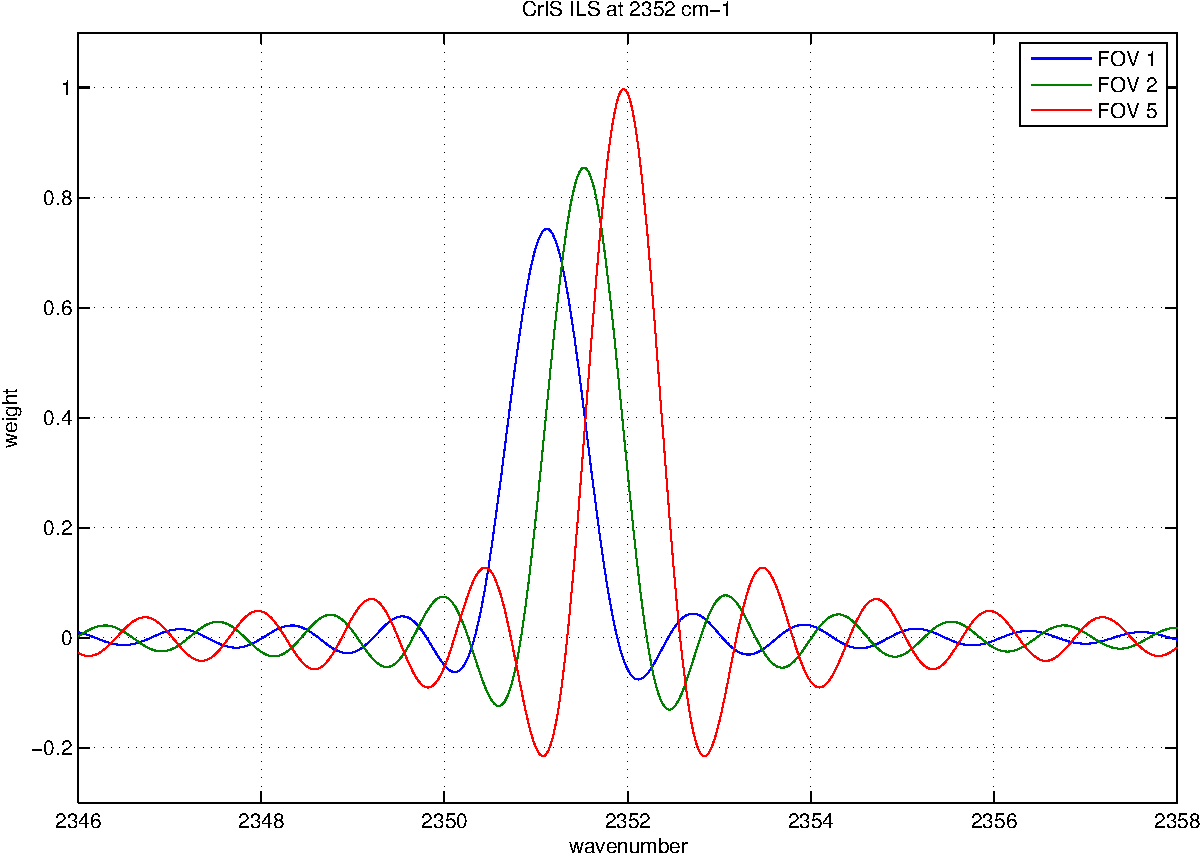
\includegraphics[scale=0.5]{figures/ILS_SW_demo.pdf}
\end{center}
\end{frame}
%----------- slide --------------------------------------------------%
\begin{frame}
\frametitle{extended interferogram apodization}

\begin{itemize}
  \item we can drop 6 points on each side of the extended resolution
    interferograms and stay very close to the {\opd} spec

 \item $(n - 12) \cdot dx =$ 1.5995 for the LW, 1.6081 for the MW,
   and 1.6001 for the SW bands, for typical metrology laser values

 \item this includes the MW band, even though that was not extended
   in the recent update

 \item apodizing (rather than dropping) these points leaves
   effective resolution within specs

 \item note that the apodized extension discussed here is distinct
   from any downstream apodization (such as Hamming) that is applied
   to user-grid radiances

\end{itemize}

\end{frame}
%----------- slide --------------------------------------------------%
\begin{frame}
\frametitle{extended interferogram apodization}
\begin{center}
  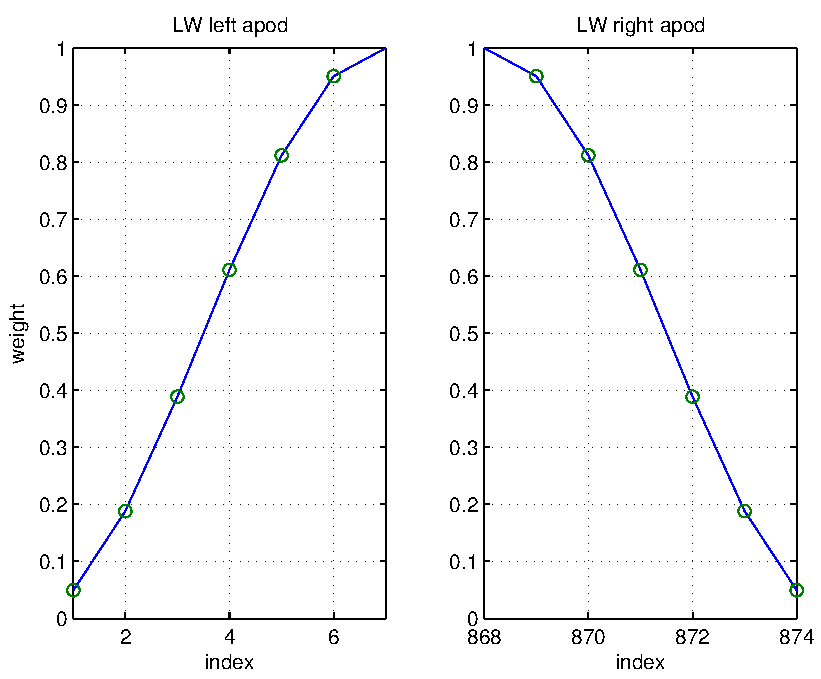
\includegraphics[scale=0.5]{figures/apod_LW.pdf}
\end{center}
edge of band details for the LW extended resolution apodization.
The apodization is symmetrical and all the weights are non-zero.
\end{frame}
%----------- slide --------------------------------------------------%
\begin{frame}
\frametitle{calibration equation notes}

\begin{itemize}
  \item most {\ccast} validation tests were done with calibration
    equations (1) and (3), but Yong and Larrabee have suggested
    moving to (2) instead of (1) for the ``ratio first'' approach

  \item the second processing filter applications gave a significant
    reduction in residuals in earlier tests, but may no longer be
    necessary

  \item runtime for the equations is similar.  The {\noaa} equation 
    is more complex but the denominator needs to be calcluated only
    once per scan

  \item equation (1) is {\ccast} calibration option ``e5'', (2) is
    ``e6'', and (3) is ``d4''.  The {\ccast} option names were set
    in earlier test rounds

  \item parameters for the {\umbc} extended res {\atbd} filter are
    chosen to match the {\noaa} high res filter as a function of
    frequency

\end{itemize}

\end{frame}
%----------- slide --------------------------------------------------%
\end{document}

